%
% FH Technikum Wien
% !TEX encoding = UTF-8 Unicode
% LTeX: language=en
%
% Erstellung von Master- und Bachelorarbeiten an der FH Technikum Wien mit Hilfe von LaTeX und der Klasse TWBOOK
%
% Um ein eigenes Dokument zu erstellen, müssen Sie folgendes ergänzen:
% 1) Mit \documentclass[..] einstellen
%    * Master- oder Bachelorarbeit
%      * Master   ... Masterarbeit
%      * Bachelor ... Bachelorarbeit
%    * Sprache (english, german, ngerman)
%    * Zitationsstandard (Harvard, IEEE) (Standard: IEEE)
%    * Biber oder BibTeX als Literaturbackend (Biber, BibTeX) (Standard: Biber)
% 2) Studiengang ausfüllen
% 3) Deckblatt, Kurzfassung, etc. ausfüllen
% 4) und die Arbeit schreiben (die verwendeten Literaturquellen in Literatur.bib eintragen)
%
% Getestet mit TeXstudio mit Zeichenkodierung utf-8 (=ansinew/latin1) und TexLive unter Ubuntu
% Zu beachten ist, dass die Kodierung der Datei mit der Kodierung des paketes inputenc zusammen passt!
% Die Kodierung der Datei twbook.cls MUSS ANSI betragen!
% Bei der Verwendung von UTF8 muss nicht nur die Kodierung des Dokuments auf UTF8 gestellt sein, sondern auch die des BibTex-Files!
%
% Bugreports und Feedback bitte per E-Mail an latex@technikum-wien.at
%
% Version V2.24 von 2024-12-19 otrebski
%
\documentclass[Master,english,IEEE]{twbook}
\usepackage[utf8]{inputenc}
\usepackage[T1]{fontenc}
\usepackage{placeins}


% bitte setzen Sie hier den Studiengang
\degreecourse{Data Science}

\addbibresource{Literatur.bib}
%% Definieren Sie hier bei Bedarf weitere Literaturdatenbanken

% Die nachfolgenden Pakete stellen sonst nicht benötigte Features zur Verfügung
\usepackage{blindtext}

%
% Einträge für Deckblatt, Kurzfassung, etc.
%
\title{Interpretable Probabilistic Electricity Load Forecasting Using Bayesian LSTM and Explainable AI Methods in Renewable Dominated Power Grids}
\author{Ing. Lucas Hausensteiner, BSc.}
\studentnumber{2410854015}
%\author{Titel Vorname Name, Titel\and{}Titel Vorname Name, Titel}
%\studentnumber{XXXXXXXXXXXXXXX\and{}XXXXXXXXXXXXXXX}
\supervisor{DI Dr. Momeni-Ortner}
%\supervisor[Begutachter]{Titel Vorname Name, Titel}
%\supervisor[Begutachterin]{Titel Vorname Name, Titel}
%\secondsupervisor{Titel Vorname Name, Titel}
%\secondsupervisor[Begutachter]{Titel Vorname Name, Titel}
%\secondsupervisor[Begutachterinnen]{Titel Vorname Name, Titel}
\place{Wien}
\kurzfassung{Diese Masterarbeit untersucht, wie Interpretierbarkeit und Unsicherheitsabschätzung in die Day-Ahead-Prognose der elektrischen Last für die österreichische Gebotszone integriert werden können. Dafür werden 15-minütige Lastdaten der ENTSO-E Transparency Platform mit Wetterdaten aus ERA5 und ECMWF kombiniert. Verglichen werden drei Modelle: Prophet, ein deterministisches LSTM und ein Bayesian LSTM. Die Datenaufbereitung umfasst die räumliche Aggregation der Wetterdaten auf Österreich, die Umwandlung akkumulativer Wettergrößen in Raten, die zeitliche Angleichung an die 15-Minuten-Auflösung und eine Verschiebung der Wetterprädiktoren um 24 Stunden zur Abbildung des Day-Ahead-Szenarios.

Die Feature-Evaluierung zeigt, dass der historische Lastverlauf der wichtigste Einflussfaktor ist. Kalendermerkmale, vor allem die Information, ob es sich um einen Werktag handelt, liefern einen starken zusätzlichen Beitrag. Zukünftige Wetterdaten verbessern die Prognose weiter, während vergangene Wetterdaten alleine weniger hilfreich sind. Das deterministische LSTM erzielt die beste Punktprognose mit einem RMSE von 341.09 MW, einem MAE von 218.39 MW und einem MAPE von 3.39 \%. Das Bayesian LSTM erreicht eine ähnliche RMSE, zeigt aber einen höheren MAE. Prophet weist deutlich höhere Fehler auf. Eine Analyse nach Tagesabschnitten zeigt außerdem, dass der Mittagsbereich für alle Modelle am schwierigsten vorherzusagen ist.

Das Bayesian LSTM kann probabilistische Prognosen erzeugen, die Unsicherheitsintervalle sind jedoch ohne weitere Kalibrierung noch nicht vollständig verlässlich. PIT-Histogramme und Intervallmetriken zeigen, dass einige Modellvarianten zu schmale Intervalle erzeugen und dadurch zu sicher wirken. Eine nachträgliche Kalibrierung verbessert die Abdeckung der unterdispersen größeren Modellvarianten, vergrößert jedoch deren Intervallbreite. Bei der kleineren Hidden-Size Variante werden die Intervalle schmaler, die Abdeckung sinkt jedoch. Die SHAP-Analyse zeigt, dass die LSTM-basierten Modelle vor allem den jüngsten Lastverlauf und den Werktagsindikator nutzen. Wettervariablen liefern eher ergänzende Information. Wiederholte SHAP-Auswertungen des Bayesian LSTM zeigen, dass die Rangfolge der wichtigsten Einflussfaktoren trotz stochastischer Gewichtssamples weitgehend stabil bleibt. Zusätzlich wurde ein Streamlit-Prototyp entwickelt, in dem Prognosen, Unsicherheitsintervalle und SHAP-Erklärungen gemeinsam betrachtet werden können. Insgesamt zeigt die Arbeit, dass interpretierbare probabilistische Lastprognosen grundsätzlich möglich sind. Die zuverlässige Kalibrierung der Unsicherheitsintervalle bleibt jedoch die wichtigste offene Herausforderung.}

\schlagworte{Elektrische Lastprognose, probabilistische Prognose, Bayesian LSTM, SHAP, Interpretierbarkeit, Unsicherheitsquantifizierung}


\outline{This thesis investigates how interpretability and uncertainty quantification can be combined in day-ahead electricity load forecasting for the Austrian bidding zone. For this purpose, 15-minute load data from the ENTSO-E Transparency Platform are combined with weather data from ERA5 and ECMWF. Three forecasting models are compared: Prophet, a deterministic LSTM and a Bayesian LSTM. The preprocessing pipeline includes spatial aggregation of weather data to Austria, conversion of accumulated weather variables into rates, temporal alignment to the 15-minute load resolution and a 24-hour shift of weather predictors to match the day-ahead forecasting setup.

The feature evaluation shows that historical load is the most important input. Calendar indicators, especially weekday information, provide a strong additional signal. Future weather covariates improve the forecast further, while past weather information alone is less useful. The deterministic LSTM achieves the best point forecast performance with an RMSE of 341.09 MW, an MAE of 218.39 MW and a MAPE of 3.39\%. The Bayesian LSTM remains close in RMSE but performs worse in MAE, while the Prophet baseline has the highest errors in this setup. A regime-wise analysis shows that the midday period is the most difficult part of the day for all models.

The Bayesian LSTM is able to produce probabilistic forecasts, but the uncertainty estimates are not fully reliable without further calibration. PIT histograms and prediction interval metrics show that some variants are underdispersed and produce intervals that are too narrow. Post-hoc calibration improves coverage for the underdispersed larger model variants, but increases their interval width. For the smaller hidden size variant, it narrows the intervals but reduces coverage. The SHAP analysis shows that both LSTM-based models mainly rely on recent load and weekday information, while weather variables play a smaller supporting role. Repeated SHAP evaluations of the Bayesian LSTM show that the overall attribution ranking remains stable under stochastic weight sampling. Finally, a Streamlit prototype demonstrates how forecasts, prediction intervals and SHAP-based explanations can be inspected in one practical interface. Overall, the thesis shows that interpretable probabilistic load forecasting is feasible, but that calibration of uncertainty estimates remains the main open challenge.}

\keywords{Electricity load forecasting, probabilistic forecasting, Bayesian LSTM, SHAP, interpretability, uncertainty quantification}

%\acknowledgements{\blindtext}

\begin{document}

\maketitle

%
% .. und hier beginnt die eigentliche Arbeit. Viel Erfolg beim Verfassen!
%
\chapter{Introduction}
\section{Motivation of the topic}
The goal of reducing greenhouse gas emissions to net-zero CO$_2$ is considered one of the greatest challenges for humanity in the upcoming decades. As a consequence, the existing energy infrastructure must undergo a deep transformation not seen before during this decarbonization phase. The resulting increase in distributed energy resources (DER) like electric vehicles and heat pumps as well as photovoltaics will evidently change existing load and power generation patterns used for electric load forecasting today \cite{hongProbabilisticEnergyForecasting2016}.

The field of energy load forecasting (ELF) is under active research due to its crucial role in modern power systems \cite{baurExplainabilityInterpretabilityElectric2024}. Accurate load forecasts support a wide range of applications including demand-response optimization, energy trading, power system scheduling, maintenance planning and capacity sizing for various stakeholders such as transmission system operators (TSO), distribution system operators (DSO), industrial consumers and building energy managers \cite{baurExplainabilityInterpretabilityElectric2024,andriopoulosShortTermElectric2021,yaprakdalMultivariateTimeSeries2023,liPowerLoadForecasting2022}. TSOs are responsible for maintaining a reliable grid and are challenged by the prospect of the changing electrical load and power generation patterns \cite{baurExplainabilityInterpretabilityElectric2024}.

Easier to understand statistical models have been historically important in forecasting, including regression-based load forecasting models as well as time series models such as ARIMA and its seasonal extension SARIMA \cite{papalexopoulosRegressionbasedApproachShortterm1990,zhangTimeSeriesForecasting2003}. These assume that electrical load can be determined by a linear combination of the previous load values and other exogenous variables \cite{andriopoulosShortTermElectric2021}. More recently, decomposition-based models such as Prophet have gained popularity as they offer flexible modelling of seasonality, trends and holiday effects while remaining interpretable \cite{bashirShortTermElectricity2022}.

Interpretability is often a vaguely used term in the literature but Baur et al. define it as the ability of humans to understand the model's decision process just by understanding the model's design \cite{baurExplainabilityInterpretabilityElectric2024}. Neural networks are nowadays gaining more attention in research because they can work with large amounts of data, have good performance and can handle complex relations of variables. Commonly used architectures in the literature include Long Short-Term Memory networks (LSTMs), XGBoost, one-dimensional Convolutional Neural Networks (1D CNNs), Support Vector Regression (SVR), as well as various ensemble and hybrid approaches that combine these methods \cite{andriopoulosShortTermElectric2021,yaprakdalMultivariateTimeSeries2023,liPowerLoadForecasting2022,bashirShortTermElectricity2022,simEXplainableAIXAIBased2022}. Yet these substantially more complex approaches do not offer insights into the model's intrinsic processes, leaving them opaque. This prompts a surge in explainability, defined as the ability to reason about the factors that influenced a model's prediction \cite{baurExplainabilityInterpretabilityElectric2024}. Currently a wide variety of model specific and agnostic explainability techniques for artificial intelligence exist (XAI). Several notable works implement such post-hoc XAI methods, like SHAP, for ELF which illustrates that these methods can be used to enhance the explainability of more complex models \cite{wuExplainableFrameworkLoad2022, liPowerLoadForecasting2022}. However, the implementation does not include uncertainty intervals, leaving operators without a clear sense of prediction risk.

This represents a problem that often gets mentioned within literature, which is the lack of a quantified uncertainty within the point estimates from interpretable models \cite{baurExplainabilityInterpretabilityElectric2024,bazionisReviewDeterministicProbabilistic2021}. TSOs must reliably assess risks and when to plan reserves. Traditional point forecasts provide a single expected load value but no information on the uncertainty or risk around that prediction. This is a reason why the domain of probabilistic load forecasting (PLF) receives growing recognition, where the models not only provide point forecasts but also depict the uncertainty in their estimates over prediction intervals or scenarios.

Generally, Baur et al. describe how the different types of PLF models can be assigned in three distinct groups. First, there are deterministic models that transform into ensemble learners when they are given different input scenarios. Second, models that implicitly learn a posterior distribution and lastly post-process a point forecast model by including residual likelihood functions \cite{baurExplainabilityInterpretabilityElectric2024}.

Although such PLF models can yield prediction intervals, they have rarely been paired with explainability techniques. Furthermore, Bayesian neural network approaches build on foundational work by Blundell et al., who introduced Bayes by Backprop as a variational method for learning probability distributions over neural network weights \cite{blundellWeightUncertaintyNeural2015}. This makes it possible to estimate predictive uncertainty through repeated sampling from the learned weight distributions. Yet integrating these uncertainty estimates with post-hoc explanations remains an open challenge in ELF.

Overall, while advances in deep learning have improved the accuracy of electricity load forecasts, especially with architectures like LSTM, they often suffer from a lack of interpretability and fail to provide reliable uncertainty estimates. This is critical for real-world decision-making in power systems. This limitation is particularly problematic for TSOs, who must make high-stakes operational and planning decisions under growing uncertainty caused by renewable energy integration, demand variability and climate conditions. Thus, there is a growing need for forecasting models that not only deliver high predictive performance but also offer interpretable insights and well-calibrated uncertainty estimates. Bridging this gap between accuracy, transparency and risk-awareness is the motivation of the thesis.

\section{Research Gap}

The literature has made progress to electricity load forecasting along two related but still only partially connected directions. First, probabilistic forecasting experiments based on Bayesian deep learning have been conducted to quantify forecast uncertainty in addition to point prediction performance. A closely related work of Xu et al. \cite{xuProbabilisticElectricalLoad2022} developed Bayesian RNN, LSTM and GRU models for probabilistic building electrical load forecasting and modeled both epistemic and aleatoric uncertainty through a dropout-based Bayesian approximation. Their results show that Bayesian recurrent forecasting for electrical load is not new in itself and that Bayesian LSTM architectures can perform well, at least in a building-level forecasting setting.

Second, other works have also shown that explainability methods such as SHAP can provide viable explanations for time-series forecasting models. Wu et al. \cite{wuExplainableFrameworkLoad2022} integrate SHAP into a deterministic LSTM-based multi-task forecasting framework in order to obtain both global and local explanations for an integrated energy system. In addition, work such as C-SHAP by Jutte et al. \cite{jutteCSHAPTimeSeries2025} suggests that SHAP explanations for time series can also be grouped at a higher conceptual level, which is relevant when low-level lag-wise attributions would otherwise become difficult to interpret. Taken together, these studies show that SHAP-based interpretation of forecasting models is an active and relevant research direction.

However, these two strands of research are still rarely brought together in one comparable framework. Xu et al. focus on probabilistic forecasting performance, lag selection and forecast horizon effects, but do not investigate post-hoc explanation stability under stochastic Bayesian forward passes. In contrast, Wu et al. demonstrate that SHAP can be useful for interpreting forecasting models, but they do not examine Bayesian probabilistic forecasting, predictive calibration, or uncertainty-aware explanation analysis. As a result, existing studies show either that Bayesian recurrent forecasting is feasible or that SHAP-based interpretation is useful, but they do not show evidence on how probabilistic neural forecasting models behave when both predictive uncertainty and explanation stability are assessed together.

This thesis addresses that gap in a deliberately focused setting. It explores day-ahead electricity load forecasting for the Austrian bidding zone at a 15-minute temporal resolution and compares Prophet, a deterministic LSTM and a Bayesian LSTM. Austria is used as a case study for a renewable-energy-dominated European grid context rather than as a universal proxy of all power systems. The main objective is not to provide a comprehensive benchmark across all forecasting horizons, market areas or model families. It also does not try to implement the full operational forecasting procedures of transmission system operators. Instead, the thesis investigates whether probabilistic forecasting and post-hoc explainability can be combined in a consistent and practically meaningful way within this specific energy system-level setting.

To the author's best knowledge, research explicitly combining Bayesian LSTM-based probabilistic load forecasting with SHAP-based analysis of explanation stability under model uncertainty remains limited.

\section{Research questions}

The core research of this thesis engages with the question of how explainability methods and uncertainty quantification can be applied to short term electricity load forecasting. 

To address this broader question, the following subquestions are explored:

\begin{enumerate}
  \item What are the main influence factors on the day-ahead load and must
  these be preprocessed in this context?
  \begin{description}
    \item[Method:] Data engineering and data analysis.
    \item[Expected Output:] Identified key drivers and a justified
    preprocessing pipeline.
  \end{description}

  \item How do probabilistic forecasts from a Bayesian LSTM compare to those
  from standard deterministic models in terms of point forecast accuracy,
  calibration, interval quality and model interpretability?
  \begin{description}
    \item[Method:] Comparative model evaluation.
    \item[Expected Output:] Quantitative and qualitative comparison of point forecast performance, probabilistic calibration, prediction interval quality and interpretability.
  \end{description}

  \item How does embedding Bayesian uncertainty into LSTM forecasts impact the
stability of post-hoc SHAP explanations, measured via empirical uncertainty
intervals over SHAP values?
  \begin{description}
    \item[Method:] SHAP-based explainability analysis under uncertainty.
    \item[Expected Output:] Assessment of explanation stability
    under probabilistic forecasting.
  \end{description}
\end{enumerate}

These research questions shall contribute to bridge the gap between advanced machine learning accuracy and operational transparency under uncertainty. 

\chapter{Methodology}


\section{Model Architectures and Implementation}

\subsection{Prophet}
Prophet is used as an interpretable statistical benchmark. As described in the work of Bashir et al. \cite{bashirShortTermElectricity2022}, a standard single Prophet model can achieve reasonable forecasting performance, while being inherently interpretable by its architecture. Although ARIMA and SARIMA models are also widely recognized standard statistical forecasting approaches, the robustness of Prophet as well as the automatic handling of seasonal patterns and trend changes make it comparably fast to deploy and verify, especially in comparison with the longer tuning process of LSTM-based models. This is why it is chosen as a standard baseline to compare against. In this work, Prophet is specified with yearly, weekly and daily seasonal components as well as six external regressors, consisting of four weather variables and two calendar indicators.

The model requires a tabular input representation in which the timestamp is stored in a column named \texttt{ds} and the target variable in a column named \texttt{y}. The merged 15-minute dataset is therefore transformed from an indexed time series into a data frame that follows this naming convention. All exogenous variables are added as additional regressor columns. In the final model specification, these regressors are the 24-hour-ahead weather variables together with the calendar indicators. Public holidays are represented as a binary exogenous regressor rather than through Prophet's native holiday calendar interface. This decision is made to be able to model a shared holiday effect across all holidays while keeping the feature representation consistent with the neural benchmark models. It also supports a more direct comparison of SHAP values across model classes, at the cost of not estimating holiday-specific effects.

Furthermore, a small grid search is performed over the most relevant Prophet hyperparameters. The evaluated search space includes the changepoint prior scale 
\(\tau_{\mathrm{cp}} \in \{0.01, 0.05, 0.06, 0.10, 0.50\}\), 
which controls the flexibility of the trend component, as also done in \cite{bashirShortTermElectricity2022}. In addition, the seasonality prior scale 
\(\tau_{\mathrm{s}} \in \{0.01, 0.10, 1.00, 10.00\}\), 
which regularizes the seasonal components and the seasonality mode 
\(m \in \{\text{additive}, \text{multiplicative}\}\), 
which determines whether seasonal and regressor effects enter the model additively or multiplicatively, are evaluated as well. The seasonal components themselves are kept fixed to yearly, weekly and daily seasonality, since these reflect the expected structure of electricity demand at 15-minute resolution.

The model assessment and hyperparameter selection are conducted with a 5-fold TimeSeriesSplit on the combined training and validation period. In each fold, Prophet is fitted only on past observations and then used to predict the corresponding holdout period from the known future regressor values. Since Prophet produces one point forecast per timestamp, its quarter-hourly predictions are regrouped into overlapping 96-step sequences so that the reported errors are evaluated on the same target horizon and MW scale as the direct multi-horizon neural models. This makes Prophet a comparable statistical baseline, but not an identical input-representation benchmark, because it does not use the same 672-step lagged-load sequence as the LSTM-based models. The hyperparameter configuration with the lowest mean cross-validation RMSE is selected. After cross-validation, the final model is refitted on the combined training and validation periods and evaluated once on the held-out test set.

\subsection{LSTM}

The deterministic neural benchmark is implemented as a sequence-to-vector LSTM in PyTorch. A multivariate lookback window of 672 time steps, corresponding to seven days at 15-minute resolution, was selected to capture one complete weekly load demand cycle while keeping model training and interpretation computationally feasible. The hidden state of the final time step is passed to a fully connected output layer that directly predicts the full 96-step day-ahead horizon. This direct multi-output definition was preferred over recursive one-step forecasting in order to avoid the accumulation of prediction errors across the horizon.

Before training, both the input features and the target load series are scaled using a robust transformation fitted on the training set only. This choice reduces the influence of outliers in the scaling process.

After scaling, the multivariate time series is rearranged into overlapping input-output sequences for training. Each input sample contains the previous 672 observations and each target sample contains the subsequent 96 load observations, corresponding to the day-ahead forecasting horizon. The resulting training sample tensors can then be passed directly to the recurrent network.

Before the final model training, several candidate feature sets were compared in a preliminary 5-fold temporal cross-validation experiment. The final experiments use the selected feature set consisting of historical load values, weekday and holiday indicators and the four 24-hour-ahead weather variables as described in section \ref{sec:feature-set-evaluation}. The hyperparameters were then optimized with Optuna in 50 trials, with validation MSE as the optimization objective. A median pruner with 10 warm-up epochs was used to stop unpromising trials early. The evaluated search space and selected configuration are summarized in Table~\ref{tabLstmHyperparameterSearch}.


\begin{table}[!htbp]
\centering
\caption{Optuna search space for the deterministic LSTM.}
\label{tabLstmHyperparameterSearch}
\begin{tabular}{lll}
\hline
Hyperparameter & Search space & Selected value \\
\hline
Hidden size & $\{64, 128, 224\}$ & 224 \\
Number of layers & $\{1, 2\}$ & 2 \\
Dropout & $[0.0, 0.25]$ if layers $>1$ & 0.15 \\
Learning rate & $[10^{-4}, 5 \cdot 10^{-3}]$ log-uniform & $3 \cdot 10^{-4}$ \\
Batch size & fixed & 128 \\
Weight decay & $[10^{-6}, 10^{-4}]$ log-uniform & $10^{-5}$ \\
\hline
\end{tabular}
\end{table}

Using the selected hyperparameters, the final model was optimized with Adam and MSE loss. Gradients were clipped to a norm of 1.0 and early stopping with a patience of 10 epochs was applied based on the validation error. The best validation state was kept for the final test evaluation.


\subsection{Bayesian LSTM}
\label{sec:bayesian-lstm}

The implementation of a Bayesian LSTM variant relies on the BLiTZ library \cite{pieroespositoBLiTZBayesianLayers2020}. It provides Bayesian layer variants for PyTorch and is used here to replace the deterministic recurrent layer by a variational Bayesian recurrent layer. The general idea is the same as in the Bayesian neural network motivation of Blundell et al. \cite{blundellWeightUncertaintyNeural2015}, where the model weights are not treated as single fixed values but as distributions that can be sampled during training and prediction. The model architecture is shown in Figure \ref{BayesianLSTMarchitercture}. 

\begin{figure}[!htbp]
\centering
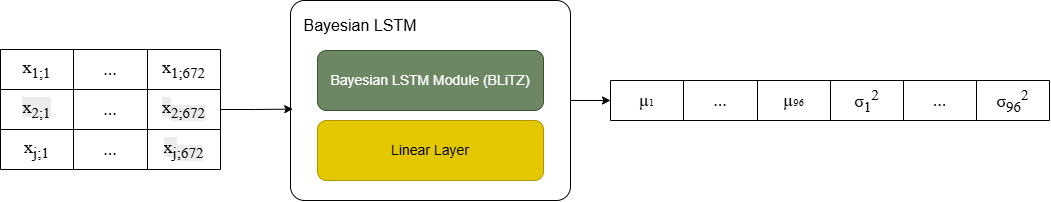
\includegraphics[width=0.9\linewidth]{PICs/BayesianLSTMArchitecture.drawio.png}
\caption{Input and output structure for the Bayesian LSTM.}\label{BayesianLSTMarchitercture}
\end{figure}

\FloatBarrier

The model receives a sequence of $x_j$ input features with lookback length $T=672$, which corresponds to seven days at a 15-minute resolution, similar to the LSTM input structure. The selected feature set contains seven input variables. These are the historical load, the weekday and holiday indicators and the four future weather variables described in Section \ref{sec:feature-set-evaluation}. In contrast to the deterministic LSTM, the Bayesian variant uses a variational LSTM layer and produces an output vector of length $2 \cdot H$ with forecasting horizon $H=96$, because both predictive means and variance parameters are required for the probabilistic objective.

Concretely, the final time step representation of the Bayesian recurrent layer is mapped by a linear output layer to 192 values. These values are split into 96 predictive means and 96 raw variance parameters. A softplus transformation combined with a small positive constant ensures that the predictive variances are only positive. This second output part represents data dependent aleatoric uncertainty, meaning the noise or variability that is present in the load signal itself. The repeated sampling of the Bayesian recurrent weights is the epistemic uncertainty, meaning uncertainty caused by the model parameters. This separation is similar in motivation to Xu et al. \cite{xuProbabilisticElectricalLoad2022}, who also modeled aleatoric and epistemic uncertainty for Bayesian recurrent load forecasting. The main difference is that Xu et al. use dropout as the variational Bayesian approximation for their Bayesian models, while this thesis uses BLiTZ Bayesian recurrent weights directly.

Training uses the sampled variational objective implemented by BLiTZ. In other words, the loss consists of a Gaussian negative log-likelihood for the prediction error and a Kullback-Leibler term from the Bayesian weight distributions. This corresponds to minimizing the negative sampled ELBO. The KL contribution is scaled by the inverse training set size using a linear warm-up during the first 30 epochs, so that the model first learns the main prediction pattern before the Bayesian regularization reaches its full weight. Adam is used as optimizer and gradients are clipped to a norm of 1.0.

Because the Bayesian model is much more expensive to train than the deterministic LSTM no broad automatic hyperparameter search is used for the final configuration. Instead, the setup is based on a small number of manual experiments. The experiments mainly varied the model size and the treatment of the KL term. Hidden sizes of 64, 96 and 128 were tried. For the KL term, a fixed weighting and a linearly increasing warm-up were compared. The final model uses the linear warm-up because it gave the model more time to learn the main prediction pattern before the Bayesian regularization reached its full strength. The final training configuration is summarized in Table \ref{tabBayesianLstmHyperparameterSearch}.

\begin{table}[!htbp]
\centering
\caption{Final handcrafted configuration of the Bayesian LSTM.}
\label{tabBayesianLstmHyperparameterSearch}
\begin{tabular}{lll}
\hline
Setting & Tried values or choice & Final value \\
\hline
Batch size & manually increased for runtime efficiency & $512$ \\
Maximum epochs & $\{40, 60, 80\}$ & $80$ \\
Hidden size & $\{64, 96, 128\}$ & $64$ \\
ELBO samples per batch & $\{3, 5\}$ & $5$ \\
Validation Monte Carlo samples & $\{5, 15, 30\}$ & $30$ \\
Test Monte Carlo samples & $\{10, 50, 100\}$ & $100$ \\
KL weighting & fixed weight and linear warm-up & linear warm-up \\
KL warm-up epochs & $\{20, 30, 40\}$ & $30$ \\
\hline
\end{tabular}
\end{table}

\FloatBarrier

Using this configuration, the final model is trained for at most 80 epochs. Validation is performed with 30 Monte Carlo forward passes per batch, while test predictions are based on 100 stochastic forward passes. The predictive mean is estimated by averaging the sampled means. The predictive variance is computed as the sum of the mean predicted variance and the variance of the sampled means. In this way, aleatoric and epistemic uncertainty are combined into one Gaussian forecast distribution for each forecast horizon.



\section{Interpretability}

Interpretability is relevant in this thesis, because it allows humans to trust the outputs of a model~\cite{InterpretableMachineLearning}. A model can either be interpretable by design or can be made interpretable by post-hoc methods \cite{baurExplainabilityInterpretabilityElectric2024}. The applied models in this thesis have very different architectures and namely recurrent neural networks are not known to be inherently interpretable by design. For this reason, the thesis uses post-hoc explainability methods to analyse which input variables influence the forecasts. A model-agnostic method is preferred because the same explanation approach can then be applied to Prophet, the deterministic LSTM and the Bayesian LSTM.

SHAP was selected as the post-hoc interpretability method because it provides local feature attributions that can be applied consistently across all considered forecasting models. This is particularly important for a multistep time-series forecasting setting, where the objective is not only to explain individual predictions, but also to compare explanations across forecast horizons and aggregate them into day-part regimes. The specific regime definition is introduced in section~\ref{sec:explainability-analysis}, where it is motivated by the observed daily demand pattern.

PDP and ICE mainly describe marginal feature-effect relationships, while SHAP decomposes each prediction into signed feature contributions relative to a baseline. This makes SHAP better suited for identifying which variables increase or decrease a specific forecast. Compared with LIME, SHAP was preferred because LIME depends on locally fitted surrogate models and random perturbations, which are less straightforward for structured sequential inputs and the explanations may vary noticeably across runs \cite{InterpretableMachineLearning}. Since the input variables in load forecasting are strongly correlated over time, PDP and ICE would also be more difficult to interpret consistently across lagged load, calendar variables and weather-based predictors. For these reasons, SHAP offers the best balance between consistency, model comparability and interpretability for the multistep forecasting used in this thesis.

Other literature has shown similar applicability of SHAP to the forecasting domain such as~\cite{chakrabortyScenariobasedPredictionClimate2021, mitrentsisInterpretableProbabilisticModel2022}, which use SHAP for local explanations of individual forecasts and for global interpretations by aggregating explanations over many data points.

In this thesis, this idea is extended to the electricity load forecasting setting and adapted to the specific structure of the implemented models. SHAP is used first on the local level to decompose selected forecasts into signed feature contributions. This shows how recent load values, calendar variables and weather information influence a single predicted horizon. For the LSTM-based models, the explanation setup groups the sequential input into feature-wise contributions across the full lookback window. This keeps the interpretation at the level of meaningful predictors instead of hundreds of individual lag positions. For Prophet, the same SHAP framework is applied to the regressor inputs of the statistical forecasting model, which makes the explanations comparable across fundamentally different model classes.

The local SHAP values are then aggregated across many forecast instances and across predefined day-part regimes in order to obtain global interpretations. This aggregation is important because electricity demand shows recurring intra-day structures and the relevance of a predictor may differ systematically between different daily regimes.

For the Bayesian LSTM, the thesis goes one step further by repeating the SHAP computation over multiple stochastic forward passes. This aims to link explainability with probabilistic forecasting. Instead of calculating only one attribution per feature and horizon, the analysis derives a distribution of SHAP values from which mean effects and empirical uncertainty intervals can be estimated. These intervals describe the variation of the explanations under stochastic Bayesian forward passes. They are therefore not classical confidence intervals from repeated data sampling. The motivation behind this is that, if the model itself expresses uncertainty through stochastic weights, then the explanations of that model should also be assessed for stability.

In the present implementation, the SHAP computation was adapted to the input structure of each forecasting model in order to obtain explanations that are computationally reasonable and semantically meaningful. For the LSTM-based models, an exact SHAP explainer is combined with a custom feature-grouped time-series masker defined on a background of $1000$ training windows sampled at one day-ahead forecast origin per day. The usage of exact SHAP is only possible because the feature set is relatively small with $F=7$ predictors. For larger feature sets, an approximate permutation-based explainer would be more realistic.

The LSTM model input has the form $N \times T \times F$, where $T$ denotes the lookback length of seven days and $F$ the number of predictors. The masker defines one coalition per predictor rather than one coalition per lagged input cell. This builds on a similar reasoning of concept-level time-series explanations, where lower-level temporal inputs are grouped into semantically meaningful units to improve interpretability \cite{jutteCSHAPTimeSeries2025}. An attribution on the level of every individual lagged cell would fragment the explanation into hundreds of strongly correlated effects and would make the exact SHAP computationally expensive. In contrast, predictor-level grouping keeps the interpretation at the level of meaningful variables such as load history, calendar information and weather inputs. Consequently, when a feature is masked, its complete history over the lookback window is replaced by the corresponding windows from the training background, while the remaining predictors are kept unchanged. This yields SHAP tensors of shape $N \times F \times H$, with $H=96$ forecast horizons for the day-ahead prediction. For a given horizon, the SHAP values together with the corresponding base value reconstruct the explained model output.

In the LSTM-based model forecasts, the regime-specific importance is obtained by slicing the $96$-step forecast into the predefined day-part intervals Night $(0$--$24)$, Morning Ramp $(24$--$40)$, Midday $(40$--$64)$, Afternoon $(64$--$80)$ and Late Evening $(80$--$96)$. Because each LSTM input already generates a complete day-ahead forecast, one forecast origin every $96$ quarter-hours is used for the grouped training background. This keeps the issue time consistent across sampled windows, reduces redundancy from overlapping rolling windows and ensures that the background samples remain representative for the SHAP calculation. This is due to the fact, when using the whole training dataset with strongly differing starting issue-times, the sampling method could result in replacing typical morning solar radiation values with values from the night which are not representative to the actual data. A total of 416 windows of the test dataset are used to calculate the global SHAP values.

For the Bayesian LSTM, the same grouped exact explainer and test windows are retained in order to keep the explanation directly comparable to the deterministic network. The SHAP computation is repeated over $30$ stochastic forward passes. In this analysis, SHAP explains the predictive mean of the Bayesian LSTM, not the predicted variance directly. The resulting SHAP array has shape $S \times N \times F \times H$ and the $2.5$th and $97.5$th percentiles of mean absolute SHAP values are reported as empirical uncertainty intervals.

For the Prophet model, SHAP is applied to the preprocessed regressors, which makes exact SHAP feasible because the model input is tabular and comparatively low-dimensional. A prediction wrapper keeps the timestamp $ds$ fixed and explains only the regressor columns. The resulting attributions therefore quantify how the exogenous variables shift the forecast at a given timestamp relative to an expected baseline value. In order to ensure a plausible data sampling, as in the LSTM SHAP calculation, Prophet instances are sampled by stratified sampling across the same day-part regimes. This comprises $10{,}000$ explained samples in total. For each explained timestamp, the SHAP background is rebuilt from training observations at the identical quarter-hour of day capped at $1{,}718$ background rows. This aims to ensure that explanations were referenced to comparable operating conditions. Because the SHAP background is sampled from training observations at the same quarter-hour of day, this yields conditional explanations relative to typical conditions at the same time of day rather than relative to one global average over all timestamps. This design is viewed as appropriate for Prophet, because it prevents structurally different night-time, morning and evening operating conditions from being mixed into a single baseline. 

Overall, these implementation choices aim to ensure that the SHAP explanation space matches the underlying model architecture in each case and that local, regime-level and probabilistic explanations remain comparable across fundamentally different forecasting approaches.


\section{Data Sources}
The data used in this thesis comprises primarily quantitative datasets from three main sources: historical electricity load data from the ENTSO-E Transparency Platform, meteorological reanalysis data from the ERA5 (ERA5-Land hourly data from 1950 to present) \cite{ERA5LandHourlyData} dataset and weather forecasts from ECMWF Open data subset \cite{OpenData2021}.

The ENTSO-E data provide sub-hourly historical electricity load for Austria, reflecting aggregate national energy consumption patterns at high-voltage levels. It is structured as numerical time series data accessible programmatically through the ENTSO-E API \cite{TransparencyPlatformRestful}. This dataset is publicly accessible and does not require additional consent from external parties. Only the data of the Austrian bidding zone, created after the split of the former bidding zone (DE-AT-LU) in October 2018 is used.

The publicly available ERA5 datasets, obtained via the Copernicus Climate Data Store (CDS) API, contain hourly weather variables such as temperature, solar radiation and wind speed. ERA5 data are provided in netCDF format and contain spatially gridded meteorological parameters. Since some finalized ERA5 datasets are available only with a latency of approximately three months, the provisional ERA5T dataset is used to bridge the gap for recent historical data. ERA5T is updated daily, but it typically only includes data up to 5-7 days before the current date. This is making it suitable for near-real-time applications while still being subject to later revisions.

For day-ahead forecasting, additional data is needed to fill in the missing gaps for the meteorological variables. This is why ECMWF numerical weather forecasts are ingested as well. ECMWF forecasts conveniently provide the meteorological predictions for the same variables with a lead time of 24 hours suitable for day-ahead applications. These data are typically available in GRIB, which are similarly spatially aggregated to generate forecasting-ready time series, as described in the following sections.

\section{Data Engineering and Preprocessing}
\subsection{Weather Variable Preprocessing}

The weather variables used in this thesis are selected because they are commonly related to electricity demand. Temperature at 2 metres (\texttt{t2m}) is included because heating and cooling demand are strongly temperature-dependent. Surface solar radiation downwards (\texttt{ssrd}) is used as an indicator for solar conditions, daylight intensity and possible photovoltaic-related demand effects. Total precipitation (\texttt{tp}) is included as a general weather condition that may influence demand behaviour. Wind speed is derived from the 10-metre wind components \texttt{u10} and \texttt{v10}, since wind conditions can describe broader weather regimes.

The wind speed feature is calculated as

\[
v_{\mathrm{wind}} = \sqrt{u_{10}^{2} + v_{10}^{2}}.
\]

Temperature is used as an instantaneous variable. Surface solar radiation downwards and total precipitation are accumulated variables and are therefore transformed into interval rates before temporal alignment.

These meteorological variables are retrieved from the Copernicus Climate Data Store and ECMWF are available at an hourly resolution on a spatial grid defined by latitude and longitude. Since the forecasting task is defined at the level of the Austrian bidding zone, these gridded fields are reduced to country-level time series before they are used for modelling. For this purpose, a spatial mask for Austria is applied to the grid and the remaining grid-cell values are averaged over the latitude and longitude dimensions for each timestamp. The result is one country-level time series per weather variable, which preserves the temporal development of the meteorological conditions while omitting spatial detail that is not required for the selected forecasting setup.

A distinction must be made between instantaneous variables, such as the temperature at two metres and accumulated variables, such as total solar radiation downwards and total precipitation. Instantaneous variables can be used directly after spatial aggregation. Accumulated variables, in contrast, first are transformed from cumulative values into hourly increments by differencing consecutive timestamps. In a subsequent step, these interval totals are normalized by the interval length in order to represent a rate over the corresponding hour. In addition, the two horizontal wind components are combined into a scalar wind-speed feature. The resulting hourly weather series are then persisted in a PostgreSQL database using a UTC timestamp representation.

\subsection{Frequency Conversion}
The target load series is available at a 15-minute resolution. Consequently, the hourly weather variables have to be aligned to the same temporal grid before they can be used as exogenous predictors. This is achieved by reindexing the hourly weather series to the 15-minute load index and forward-filling the most recent hourly observation across the four quarter-hour intervals contained in each hour, as illustrated in Figure \ref{ForwardFill}. In this way, all features share a common time axis while the weather information remains temporally consistent within the hour.

\begin{figure}[!htbp]
\centering
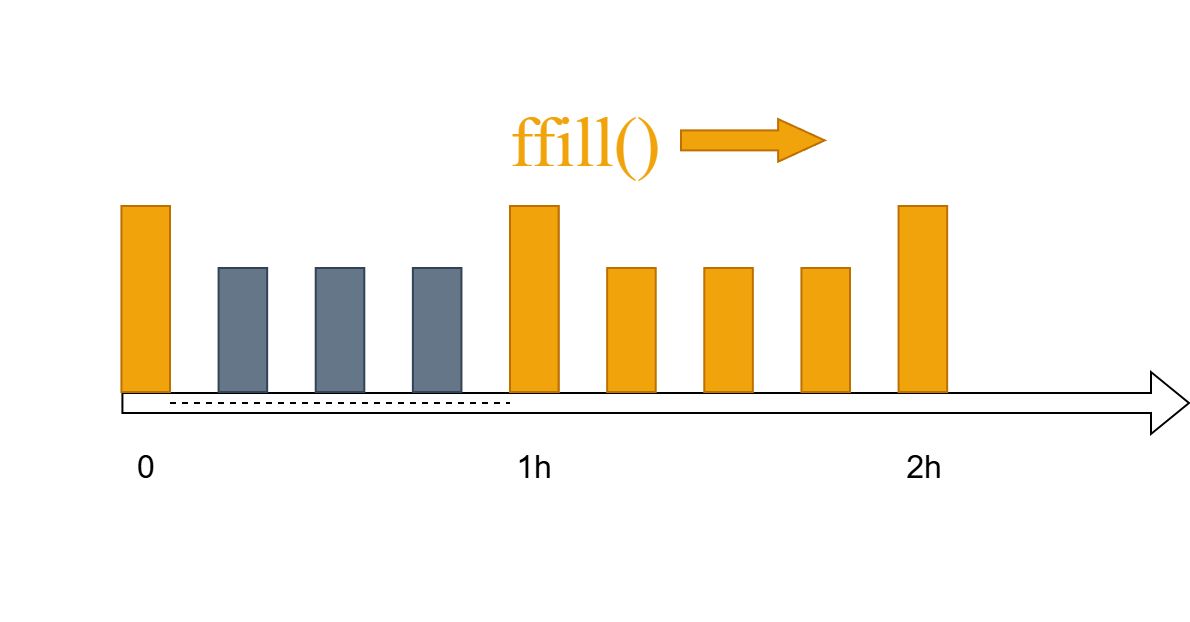
\includegraphics[width=0.5\linewidth]{PICs/FFill.drawio.png}
\caption{Forward filling of hourly weather variables to align them with the 15-minute load series.}\label{ForwardFill}
\end{figure}

\FloatBarrier

To reflect the day-ahead forecasting task, the weather variables are then shifted by 24 hours, corresponding to 96 quarter-hour steps. Thus, for a forecast origin at time $t$, the feature vector contains historical load information together with meteorological forecasts associated with the target period up to $t + 24$ hours. These weather inputs refer to forecast values available before or at the forecast origin, not the realized future ERA5 observations in order to avoid information leakage. Finally, the weather variables are merged with the load series on the common timestamp index and enriched with calendar indicators. The model-specific representation of this merged dataset is described in the corresponding model subsections below.

\subsection{Calendar Feature Engineering}
Calendar variables are derived directly from the timestamp index. The weekday indicator is defined as

\[
x_{\mathrm{weekday}}(t) =
\begin{cases}
1, & \text{if } t \text{ is Monday to Friday},\\
0, & \text{otherwise}.
\end{cases}
\]

The holiday indicator is defined as

\[
x_{\mathrm{holiday}}(t) =
\begin{cases}
1, & \text{if } t \text{ is an Austrian public holiday},\\
0, & \text{otherwise}.
\end{cases}
\]

For experiments using cyclic calendar encodings, periodic variables are transformed into sine and cosine pairs:

\[
x_{\sin}(t) = \sin\left(2\pi \frac{k(t)}{P}\right),
\qquad
x_{\cos}(t) = \cos\left(2\pi \frac{k(t)}{P}\right),
\]

where \(k(t)\) is the position within the period and \(P\) is the period length. This encoding is applied to time of day, day of week and day of year.

\section{Experiment Tracking}

All experiments are run locally using Jupyter Notebooks. To ensure reproducibility, the intermediate metrics and final models are logged to a local MLflow server instance. For transparency and reproducibility, the implementation, notebooks and supporting project files are publicly available in the project repository \cite{lucashausiLucasHausiProbabilisticloadforecastproject2026}.
 

\section{Evaluation Framework}

All models are evaluated on a test period that preserves the temporal ordering of the data in order to avoid information leakage from future observations. The preprocessed dataset is split into training, validation and test periods using a 70/15/15 ratio. The training set contains 164,214 observations from 2018-10-01 00:00 UTC to 2023-06-15 13:00 UTC. The validation set contains 39,863 observations from 2023-06-15 13:15 UTC to 2024-08-11 18:30 UTC. The test set contains 39,863 observations from 2024-08-11 18:45 UTC to 2025-10-09 00:00 UTC. The RobustScaler is fitted on the training period only and then applied to the validation and test periods.

The point forecast quality is evaluated using RMSE, MAPE and MAE on the original MW scale also to compare against other literature.

To assess the possible covariates for predicting future load, several candidate feature sets were defined to reflect different modelling assumptions, including load-only, load with calendar indicators, load with past weather, load with future weather, combinations of past and future weather and variants with cyclic calendar encodings. Each feature set is evaluated with the same architecture and initial training configuration, so that differences in performance can be attributed primarily to the input representation. The feature set with the best balance between complexity and performance is then used for the subsequent model development, final model comparison and explainability analysis.

For the probabilistic Bayesian LSTM, the evaluation is extended beyond point accuracy. Chen et. al. suggest that PIT histograms are used as a calibration diagnostic~\cite{chenEvaluationProbabilisticElectricity2024}. For each forecasted value, the predictive cumulative distribution function is evaluated at the observed load value. A well-calibrated probabilistic model should produce PIT values that are approximately uniformly distributed. However, PIT histograms mainly assess calibration and do not measure the sharpness or practical usefulness of prediction intervals by themselves.

Therefore, the probabilistic evaluation is complemented by the prediction interval coverage probability (PICP) and the mean prediction interval width (MPIW), following the interval-based comparison used by Xu et al.~\cite{xuProbabilisticElectricalLoad2022}. PICP measures the share of observed load values that fall inside the predicted interval, while MPIW measures the average width of these intervals. Both metrics are interpreted together, because high coverage is only useful if the intervals are not very large, while narrow intervals are only meaningful if they still achieve an adequate coverage.

\chapter{Results}

\section{Feature Set Evaluation}
\label{sec:feature-set-evaluation}

There were quite different features proposed by literature for this forecasting problem. Summarized, the main contributing factors are identified as calendar features like holiday indicators and weather covariates \cite{yaprakdalMultivariateTimeSeries2023, papalexopoulosRegressionbasedApproachShortterm1990, baurExplainabilityInterpretabilityElectric2024, liPowerLoadForecasting2022}. To understand how these covariates influence day-ahead load forecasting in the Austrian bidding zone, a comparative evaluation of alternative input representations was conducted.

The evaluated feature sets were built from different combinations of load history, calendar information and weather variables. Load history was used as the basic input in all experiments. Additional variants added simple calendar indicators such as weekday, weekend and holiday flags. Weather information was tested either as past weather values, 24-hour-ahead weather covariates or as a combination of both. Some variants also included cyclic calendar encodings for time of day, day of week and day of year. This setup makes it possible to compare how much each group of features contributes marginally to the forecast quality, while keeping the forecasting architecture fixed across experiments.

\begin{figure}[!htbp]
\centering
\includegraphics[width=1\linewidth]{PICs/feature_set_evaluation.png}
\caption{Feature set evaluation results.}\label{FeatureSetEvaluation}
\end{figure}

The Figure \ref{FeatureSetEvaluation} displays the cross-validated results of the feature evaluation experiments.

Upon examining the results, it is evident that calendar features improve the forecast compared to the load-only baseline. The load-only feature set reaches a cross-validated RMSE of 429.34 MW, while adding basic calendar indicators reduces the RMSE to 380.19 MW. Adding cyclic calendar encodings gives a similar result with an RMSE of 375.28 MW. This indicates that the cyclic representation provides only a small additional improvement over the simpler calendar indicators. This is not the case when comparing future and past weather information. Adding past weather to the load-only setup worsens the RMSE from 429.34 MW to 449.30 MW, while adding future weather improves it to 409.27 MW. The same pattern is visible when calendar features are included: load, calendar and past weather reach 421.87 MW, whereas load, calendar and future weather reach 360.54 MW. This shows that 24-hour-ahead weather covariates provide substantially more predictive value than historical weather data alone.

A key constraint in the feature set selection is the total number of features, due to the computational complexity of SHAP calculations in the forecast interpretation section. Consequently, the selected feature set must balance performance and complexity. The lowest RMSE was 341.18 MW for the feature set including all variations of predictors. However, the selected feature set with historical load, future weather covariates and basic calendar indicators reached an RMSE of 360.54 MW. This corresponds to a penalty of 19.37 MW, or about 5.7\%, while keeping the feature space simpler and the later SHAP analysis more feasible.


\section{Point Forecast Quality}

The following section discloses the model comparison in terms of point forecast performance. The overall performance results are shortly summarized in Table \ref{tabPointForecast}. The deterministic LSTM achieves the lowest errors, with an RMSE of 341.09 MW, an MAE of 218.39 MW and a MAPE of 3.39\%. The Bayesian LSTM performs slightly worse, with an RMSE of 353.59 MW, an MAE of 250.21 MW and a MAPE of 3.79\%. Relative to the deterministic LSTM, this corresponds to an increase of about 3.6\% in RMSE and 14.6\% in MAE. The Prophet baseline has higher errors in this benchmark, with an RMSE of 521.33 MW, an MAE of 418.77 MW and a MAPE of 6.57\%. For reference, the average observed load in the dataset is 6,932 MW, based on the exploratory data analysis from October 2025.

These results suggest that the recurrent neural architectures were able to make use of recent temporal dependencies through the 672-step lagged input sequence. Prophet remains easier to interpret by design and provides a useful decomposition-based statistical baseline, although its input representation differs from the sequential representation used by the recurrent models.


Despite the differences between deterministic and Bayesian training, both LSTM-based model's remain in a similar performance range, with RMSE values differing by only 12.50 MW. This suggests that the recurrent architecture itself is the main driver of point forecast performance, while the Bayesian extension mainly adds uncertainty information at the cost of a moderate reduction in point accuracy.

\begin{table}[!htbp]
\centering
\caption{Forecasting performance of the evaluated models on the held-out test set (unscaled).}
\label{tabPointForecast}
\begin{tabular}{| p{0.20\linewidth} | p{0.20\linewidth} | p{0.20\linewidth} | p{0.20\linewidth} |}
\hline
Model & RMSE Overall & MAE Overall & MAPE Overall \\\hline
Bayesian LSTM ($hidden size = 64$) & 353.586 & 250.205 &  3.79\% \\
LSTM & 341.090 & 218.390 & 3.39\% \\
Prophet & 521.325 & 418.771 & 6.57\% \\\hline
\end{tabular}
\end{table}

The Bayesian LSTM was trained with a Gaussian negative log-likelihood loss instead of a pure MSE loss, as described in Section~\ref{sec:bayesian-lstm}. This allowed the model to predict both the expected load and a predictive variance. Compared to the earlier MSE-based version, the overall RMSE improved from 368.98 MW to 353.59 MW. With this adaptation, the final version not only represents epistemic uncertainty through stochastic weight sampling, but also models aleatoric uncertainty through the predicted variance.

Figure \ref{ForecastComparisson} illustrates sample day-ahead predictions over one winter week and one summer week from the test period. The individual day-ahead predictions are concatenated to provide a continuous view of the forecast trajectory. It is used as an illustrative example of model behaviour and not as a full seasonal performance evaluation.

\begin{figure}[!htbp]
\centering
\includegraphics[width=1\linewidth]{PICs/normal_weeks_plot.png}
\caption{Forecasting comparison for the different models.}\label{ForecastComparisson}
\end{figure}

\FloatBarrier

In this example above all models reproduce the general daily structure, but they show visible deviations around the midday part of the load curve. This also motivates the regime-wise explainability analysis, where the forecast horizon is grouped into day-part regimes.

In addition to the overall error metrics, the forecast errors are analysed by the day-part regime. This is useful because electricity load is not equally difficult to predict across the full day-ahead horizon. Periods with stronger ramps or less regular demand patterns may lead to higher forecast errors than more stable periods. The MAE is grouped into the same regimes that are later used for the SHAP analysis.

\begin{table}[!htbp]
\centering
\caption{MAE by day-part regime in MW.}
\label{tabDayPartMAE}
\begin{tabular}{| l | r | r | r |}
\hline
Regime & Bayesian LSTM & LSTM & Prophet \\
\hline
Night & 193.85 & 202.52 & 369.07 \\
Morning Ramp & 362.02 & 322.46 & 472.99 \\
Midday & 432.79 & 368.66 & 528.92 \\
Afternoon & 178.26 & 201.88 & 328.78 \\
Late Evening & 93.61 & 133.48 & 363.68 \\
\hline
\end{tabular}
\end{table}

Table \ref{tabDayPartMAE} shows that the Midday regime has the highest MAE for all three models. The Bayesian LSTM reaches an MAE of 432.79 MW, the deterministic LSTM reaches 368.66 MW and Prophet reaches 528.92 MW in this regime. This supports the visual inspection from Figure \ref{ForecastComparisson}, in which the models show visible deviations around the midday part of the load curve. The Morning Ramp appears challenging as well. Especially for the Bayesian LSTM and Prophet. In contrast, the Late Evening regime shows the lowest errors for both LSTM-based models, with 93.61 MW for the Bayesian LSTM and 133.48 MW for the deterministic LSTM. Overall, the deterministic LSTM performs best in the more difficult Morning Ramp and Midday regimes, while the Bayesian LSTM performs better in the Night, Afternoon and Late Evening regimes.

Another key insight is the pattern when the forecast errors are grouped by weekday. Figure \ref{WeekdayErrorComparisson} shows the signed forecast errors by weekday, where positive values indicate underprediction and negative values indicate overprediction.

\begin{figure}[!htbp]
\centering
\includegraphics[width=1\linewidth]{PICs/performance_weekday.png}
\caption{Error comparison per weekday.}\label{WeekdayErrorComparisson}
\end{figure}

\FloatBarrier

This indicates that Prophet has a larger spread of prediction errors on the weekends than on weekdays. This is especially visible on Saturday and Sunday, where the interquartile range and the outliers are larger than for the LSTM-based models. For the statistical comparison, the absolute forecast error is used. The grouped Prophet error statistics are shown in Table \ref{tabWeekdayWeekendErrors}.

\begin{table}[!htbp]
\centering
\caption{Grouped Prophet absolute error statistics by weekday/weekend regime in MW.}\label{tabWeekdayWeekendErrors}
\begin{tabular}{| l | r | r | r | r |}
\hline
Regime & Mean & Median & Std & Count \\
\hline
Weekday & 383.72 & 323.05 & 290.34 & 28\,513 \\
Weekend & 506.58 & 457.92 & 340.76 & 11\,350 \\
\hline
\end{tabular}
\end{table}

The Prophet model has higher absolute errors on weekends. The mean absolute error increases from 383.72 MW on weekdays to 506.58 MW on weekends, while the median increases from 323.05 MW to 457.92 MW. A Mann-Whitney U test comparing weekday and weekend absolute error distributions yields a p-value of $4.55\times 10^{-242}$, which indicates a statistically significant difference between the two groups.

One possible explanation is that the Prophet's deterministic seasonal decomposition does not fully capture the structural weekend regime shift in Austrian load demand. Weekend load behaviour may include non-linear dependencies or regime-specific patterns that are better modeled by the more flexible LSTM-based models. The stronger spread of positive Prophet errors in Figure \ref{WeekdayErrorComparisson} also indicates that Prophet tends to underpredict in some weekend periods.


Table \ref{tabTrainingTimes} shows the observed training times for the final model runs. These values refer to one training run per model and do not include the full cross-validation or hyperparameter search time. The Bayesian LSTM required the longest training time with 2.8 days, while the deterministic LSTM was trained in 3.1 hours and Prophet was fitted in 17.9 minutes.

This in turn clearly became a bottleneck during the experimentation phase, as it reduced the speed of model development and evaluation. Longer training times per experiment meant that fewer configurations could be tested, which restricted both tuning and rapid iteration on new ideas.

\begin{table}[!htbp]
\centering
\caption{Training times of the final model runs.}
\label{tabTrainingTimes}
\begin{tabular}{| p{0.35\linewidth} | p{0.44\linewidth} |}\hline
Model & Training Time\\\hline
Bayesian LSTM & 2.8 days\\
LSTM & 3.1 hours\\
Prophet & 17.9 minutes\\\hline
\end{tabular}
\end{table}

\section{Probabilistic Forecast Quality and Uncertainty}

The PIT histogram is a viable method to assess the calibration of probabilistic predictions. For this thesis, the CDF values are derived from repeated stochastic forward passes of the Bayesian LSTM on the test data. For each forecast horizon, the model outputs a predictive mean and a variance parameter, which together define a Gaussian predictive distribution after enforcing positivity of the variance. By sampling the model multiple times, a Monte Carlo approximation of the predictive distribution is obtained. The PIT value for a realized observation is then calculated by evaluating the corresponding predictive CDF at the observed load value and averaging these probabilities across the sampled predictive distributions. This yields one PIT value per forecasted target, from which the calibration histogram is constructed. In the ideal case, the PIT values $u = F_Y(y)$ are uniformly distributed $u \sim \mathcal{U}(0,1)$. Deviations from this benchmark provide information about the type of miscalibration.


Figure \ref{figPITValues} shows the PIT histogram of the selected Bayesian LSTM configuration with hidden size 64. It indicates a systematic skewness by a strong clustering of CDF values in the area around 0.0 as well as a lack of values in the area around 1.0. This suggests that the model tends to overpredict the actual load. Furthermore, the hump around the centre also indicates that the predictive distribution is not well fitted.

\begin{figure}[!htbp]
\centering
\includegraphics[width=0.5\linewidth]{PICs/pit_before_retraining.png}
\caption{PIT values of the Bayesian LSTM ($hidden size = 64$).}\label{figPITValues}
\end{figure}

\FloatBarrier

As a follow-up experiment, the Bayesian LSTM was retrained with larger hidden sizes in order to examine the effect of larger capacity not only on point forecast performance, but also on the calibration plot. Figure \ref{figPITValuesRetraining} depicts the PIT histograms for hidden sizes 96 and 128. The skewness is reduced compared to the initial model, but a new problem remains visible. Both histograms show a U-shaped pattern, which indicates that the predictive distributions are underdispersed. In practical terms, the model produces intervals that are too narrow and therefore expresses too much certainty. The larger model variants therefore improve the shape of the PIT histogram, but they still do not provide satisfactory calibration.



\begin{figure}[!htbp]
\centering
\includegraphics[width=1\linewidth]{PICs/pit_after_retraining_combined.png}
\caption{PIT values of the Bayesian LSTM after retraining: left ($hidden size = 96$) and right ($hidden size = 128$).}\label{figPITValuesRetraining}
\end{figure}

\FloatBarrier

The interval-based metrics in Table \ref{tabProbabilisticIntervals} support this interpretation. For a 95\% prediction interval, the PICP should be close to 0.95, while the MPIW should remain as small as possible. The hidden-size 64 model reaches a PICP of 0.9465, which is close to the nominal level, but this comes with wide intervals of 1318.81 MW. The hidden-size 96 and 128 models have lower raw coverage values of 0.8649 and 0.8909. This confirms that the larger models are under-covering the observations, which is consistent with the U-shaped PIT histograms.

\begin{table}[!htbp]
\centering
\caption{Raw and calibrated 95\% prediction interval quality of the Bayesian LSTM variants.}
\label{tabProbabilisticIntervals}
\begin{tabular}{| l | r | r | r | r |}
\hline
Model variant & Raw PICP & Raw MPIW (MW) & Cal. PICP & Cal. MPIW (MW) \\
\hline
Hidden size 64 & 0.9465 & 1318.81 & 0.9224 & 1173.24 \\
Hidden size 96 & 0.8649 & 929.49 & 0.9311 & 1243.04 \\
Hidden size 128 & 0.8909 & 1238.22 & 0.9290 & 1441.37 \\
\hline
\end{tabular}
\end{table}

An additional post-hoc calibration experiment was conducted on the Bayesian LSTM by fitting per-horizon affine corrections to the predictive mean and variance on the validation set and applying these corrections to the test forecasts. Figure~\ref{figPITValuesCalibration} shows the effect of this calibration step for the hidden-size 96 model.


\begin{figure}[!htbp]
\centering
\includegraphics[width=1\linewidth]{PICs/pit_calibration.png}
\caption{PIT after the calibration experiment of the Bayesian LSTM (hidden size = 96).}\label{figPITValuesCalibration}
\end{figure}

 
The calibration step reduces the U-shaped pattern and therefore improves the calibration of the hidden-size 96 model. This is also visible in Table \ref{tabProbabilisticIntervals}, where the 95\% PICP increases from 0.8649 to 0.9311. However, the improvement in coverage is achieved by increasing the average interval width from 929.49 MW to 1243.04 MW. A similar pattern is visible for the hidden-size 128 model. For the hidden-size 64 model, calibration narrows the intervals but also reduces coverage from 0.9465 to 0.9224. Overall, calibration helps most for models that are clearly underdispersed, but it does not improve all variants in the same way.

These results show that the Bayesian LSTM can produce probabilistic forecasts, but the raw predictive distributions are not reliably calibrated across model variants. The PIT histograms reveal a distributional miscalibration, while the PICP and MPIW values show the practical effect on prediction interval coverage and width.

However, the main objective of this thesis is to assess whether the Bayesian LSTM itself provides well-calibrated probabilistic forecasts and whether its predictions can be interpreted consistently using SHAP-based feature attributions. Integrating a post-hoc calibration into the final system would have complicated this interpretation, because the reported forecast distribution would partly come from the calibration step rather than from the neural network itself. In particular, the current SHAP analysis explains the predictive mean generated by the model, whereas calibrated uncertainty intervals depend on an additional transformation that is not directly represented in the attribution workflow.


Calibration is therefore reported as an additional experiment and is not included in the final deployed pipeline. For the subsequent experiments, the Bayesian LSTM with a hidden size of 64 is used because its raw 95\% prediction interval coverage is closest to the nominal level, although its PIT histogram still indicates distributional miscalibration.



\section{Explainability Analysis}
\label{sec:explainability-analysis}

The explainability analysis was conducted using SHAP-based global feature attributions in order to assess which input variables drive forecasts of the different model classes in different regimes. Since the forecast horizon covers a full day, the analysis is grouped into day-part regimes. Relevant regimes are identified based on typical load demand patterns as can be seen in Figure~\ref{figElectricityDemandPattern}. 

\begin{figure}[!htbp]
\centering
\includegraphics[width=0.8\linewidth]{PICs/daily_demand_pattern.png}
\caption{Daily electricity demand pattern by seasonal decomposition.}\label{figElectricityDemandPattern}
\end{figure}

\FloatBarrier

The daily seasonal component shows clearly distinguishable phases over the course of the day, including a low-demand night period, a pronounced morning ramp, a local midday minimum, a renewed increase in the late afternoon and evening and a subsequent decline overnight. For this reason, the forecast horizon is grouped into the five day-part regimes Night, Morning Ramp, Midday, Afternoon and Late Evening. Aggregating SHAP values within these regimes makes the explanations easier to interpret, because feature effects can be compared for periods with different operational demand characteristics instead of only at isolated quarter-hourly steps. Since the following plots report mean absolute SHAP values, they describe the average attribution of a feature, not the direction of its effect. The signed effects can be inspected in the detailed analysis view of the prototype user interface, which is later discussed in section~\ref{sec:deployment-concept}.

For the deterministic LSTM, the mean SHAP contributions in Figure \ref{figGlobalSHAPLSTM} show that the actual load has the largest average attribution magnitude across all forecast regimes, suggesting that the recent load history is the driver of the LSTM forecasts. The second highest attribution is accounted to the calendar-related feature indicating if it is a weekday, which seems to make it viable as a secondary signal. Both the load and weekday indicator seem to have a higher attribution around the Morning Ramp and Midday regimes, suggesting that the model relies on these features forecasting the relatively more complex midday pattern. The weather-related predictors show a smaller attribution magnitude in this setup.

\begin{figure}[!htbp]
\centering
\includegraphics[width=0.8\linewidth]{PICs/shap_regimes_lstm.png}
\caption{Global Mean SHAP values for the LSTM model.}\label{figGlobalSHAPLSTM}
\end{figure}

\FloatBarrier

A key experiment of this thesis was to examine the stability of the SHAP-based feature attributions for the selected Bayesian LSTM configuration with hidden size 64 across multiple stochastic weight samples. This means the models weights are randomly sampled and kept fixed for every SHAP evaluation. In this way, each explanation corresponds to a deterministic model instance, while the variation across runs reflects the uncertainty invoked by Bayesian weight sampling. Figure \ref{figGlobalSHAPBaysianLSTM} depicts the resulting regime-wise mean absolute SHAP values for 30 sampled model instances, with the upper and lower bands indicating the spread across runs. Overall, the attribution hierarchy is quite consistent across sampled weight configurations and closely resembles that of the deterministic LSTM. The actual load is the dominant forecast driver in all regimes, followed by the weekday indicator, while the weather variables contribute comparatively little. This suggests that the Bayesian weight uncertainty does not fundamentally alter the ranking of the most influential predictors.

\begin{figure}[!htbp]
\centering
\includegraphics[width=0.8\linewidth]{PICs/shap_regimes_bayesian.png}
\caption{Global Mean SHAP values for the Bayesian LSTM model.}\label{figGlobalSHAPBaysianLSTM}
\end{figure}

\FloatBarrier

Furthermore, a closer analysis of the regime-wise results shows that the attribution band of the weekday indicator is wider during the Morning Ramp, Midday and Afternoon regimes. This suggests that the importance of weekday information is more sensitive to the sampled weight configuration in periods with stronger variability in daily demand structure. In contrast, the attribution band of the actual load remains comparatively stable across most regimes and widens mainly in the Afternoon regime. A possible interpretation is that the reliance of the model on recent load history is likely robust overall, but becomes more uncertain during the transition from midday demand to the evening period.

\FloatBarrier

\begin{figure}[!htbp]
\centering
\includegraphics[width=0.8\linewidth]{PICs/shap_regimes_prophet.png}
\caption{Global Mean SHAP values for the Prophet model.}\label{figGlobalSHAPProphet}
\end{figure}


For Prophet, the aggregated SHAP attribution explanation differs substantially because the model does not rely on lagged load values in the same way as the recurrent architectures. Instead, the attributions are dominated by the exogenous regressors and calendar indicators that were directly added to the model. 

At the same time, it should be stated again that the SHAP analysis in this thesis only captures the contribution of the explicit input variables, but not Prophet's internal model components such as trend, weekly seasonality and daily seasonality components. This restriction was applied deliberately in order to maintain comparability with the LSTM-based models for which the interpretation is likewise based on the provided input features rather than on internal latent representations. The internal patterns learned by Prophet can still be examined separately through the model's native component plots, such as trend and seasonality visualizations.

Within the comparable SHAP framework, as shown in Figure \ref{figGlobalSHAPProphet}, temperature is the most influential feature across all regimes. This indicates that it is the primary external driver of the Prophet forecasts. The weekday indicator is the second most important contributor and remains comparatively stable across the different day-part regimes, which is consistent with the weekly structure observed in the demand data. Holiday effects contribute less strongly, while the remaining weather variables, especially wind speed and precipitation, contribute only marginally. Solar radiation shows a more regime-dependent importance, with larger SHAP values during the Morning Ramp and Midday periods and a clear decline in the Late Evening regime. Overall, the Prophet explanations suggest that the model relies mainly on structured calendar effects and a small number of dominant external drivers.

The computational cost of the SHAP-based explainability analysis differs substantially across the evaluated models. Table \ref{tabShapTimes} shows the resulting computation times of the global SHAP analysis.


\begin{table}[!htbp]
\centering
\caption{SHAP evaluation times of the evaluated models.}\label{tabShapTimes}
\begin{tabular}{| p{0.35\linewidth} | p{0.44\linewidth} |}\hline
Model & SHAP Evaluation Time\\\hline
Bayesian LSTM & 664 min 17 s\\
LSTM & 167 min 37 s\\
Prophet & 36 min\\\hline
\end{tabular}
\end{table}

Prophet has the lowest evaluation time due to its simpler additive structure and the absence of sequential dependencies. It is noticeable that the deterministic LSTM requires more computation, reflecting the higher complexity of recurrent architectures and the need to evaluate longer input sequences. In contrast, the Bayesian LSTM has the highest computational cost mainly due to the repeated SHAP evaluations over multiple stochastic forward passes in order to capture epistemic uncertainty.

It is important to note that the increase in computation time is not proportional to the number of sampled model instances. Although 30 stochastic forward passes were used, the total runtime did not increase linearly by a factor of 30 compared to the deterministic LSTM. Furthermore, since global SHAP values are typically computed only once per trained model for analysis rather than during iterative model development, the additional computational cost of the Bayesian approach remains practically feasible. 

In addition, local SHAP explanations for individual forecasts require approximately 1-3 minutes per instance. This is still considered feasible when computed once directly after the forecasts are generated for a post-hoc analysis later in that day.

Overall, the explainability results are consistent with the forecasting performance observed in the feature set benchmark. The LSTM and Bayesian LSTM derive most of their predictive strength from the recent load history and calendar effects, which is plausible for high-frequency electricity demand forecasting. Weather variables are informative, but their role is mainly complementary.

\section{Deployment Concept}
\label{sec:deployment-concept}

The deployment concept of the prototype is focused on demonstrating how the proposed forecasting approach could be integrated into a practical decision-support application. The primary objective is to provide an interface through which forecasts can be generated, inspected and interpreted in an accessible manner. The prototype is not intended to replace an operational TSO forecasting system, but to show how the developed models and explanations could be used in a practical workflow. For this purpose, a Streamlit-based frontend was selected, as it enables fast development and deployment of interactive Python applications.

The workflow starts with the user selecting the bidding zone and the forecast period in the frontend and starting the forecast. The prototype then displays the historical load data together with the generated forecasts of Prophet, the deterministic LSTM and the Bayesian LSTM. For the Bayesian LSTM, the forecast view also includes the 95\% prediction interval. This makes it possible to compare the point forecasts of all models and to inspect the uncertainty estimate of the probabilistic model in the same view. An example of this forecast view is shown in Figure~\ref{figPrototypeForecast}.

\begin{figure}[!htbp]
\centering
\includegraphics[width=1\linewidth]{PICs/prototype_forecast.png}
\caption{Forecast view of the prototype showing historical load, model forecasts and the Bayesian LSTM prediction interval.}
\label{figPrototypeForecast}
\end{figure}

The second part of the prototype focuses on interpretation. The user can select the model and the type of explanation view. The day-part view groups the SHAP explanations into the meaningful regimes such as Night, Morning Ramp, Midday, Afternoon, Late Evening as defined earlier. This allows the user to inspect which input variables are most important for a selected part of the forecast horizon. Figure~\ref{figPrototypeRegime} shows an example where the explanation is displayed for the Morning Ramp.

\begin{figure}[!htbp]
\centering
\includegraphics[width=1\linewidth]{PICs/prototype_forecast_regime.png}
\caption{Day-part interpretation view of the prototype.}
\label{figPrototypeRegime}
\end{figure}

In addition to the grouped view, the prototype also provides a timestep-level interpretation. In this view, the user selects a specific forecast timestamp and the interface shows the local feature contributions for this point in time. The signed SHAP values indicate whether a feature supports a higher or lower load forecast. This is useful because the global mean absolute SHAP values in the results section only show feature importance, while this view also shows the direction of the effect as well as the uncertainty in the case of the Bayesian LSTM. An example is shown in Figure~\ref{figPrototypeTimestep}.

\begin{figure}[!htbp]
\centering
\includegraphics[width=1\linewidth]{PICs/prototype_interpretation_time.png}
\caption{Timestep-level interpretation view with signed feature contributions.}
\label{figPrototypeTimestep}
\end{figure}

The overview interpretation provides a summary over the whole forecast day. This view is intended to give a quick impression of which features are most relevant for the selected model and forecast period. Figure~\ref{figPrototypeOverview} shows this overview for the Prophet model.

\begin{figure}[!htbp]
\centering
\includegraphics[width=1\linewidth]{PICs/prototype_interpretation_overview.png}
\caption{Whole-day interpretation overview in the prototype.}
\label{figPrototypeOverview}
\end{figure}

The frontend is connected to a FastAPI backend, which acts as the central orchestration layer and provides the data and forecasting results required by the user interface. At the core of the system lies a modular Python package whose main functionality is implemented through dedicated service components. These services encapsulate the logic for data ingestion, preprocessing and persistence and are invoked by the backend in response to frontend requests. The services interact with the ENTSO-E Transparency Platform, the ECMWF API for weather forecasts and the Copernicus Climate Data Store for ERA5 data retrieval.

The data refresh workflow is handled through the command-line interface of the package. It defines commands for fetching electricity load data, retrieving historical weather data, obtaining forecast weather inputs and storing all processed datasets in a PostgreSQL database. On top of these commands, PowerShell scripts are provided to execute the predefined workflows for the most recent required dates. In a productive environment, these scripts could either be triggered manually or scheduled automatically, for example via cron jobs or comparable task schedulers. This would ensure that the latest load and weather inputs are available before a new forecast is generated.

The forecast generation workflow uses the stored data as input for the trained models. The backend retrieves the required feature window from the database, loads the selected model and creates the 96-step day-ahead forecast. The trained models and experiment results are tracked with MLflow, which allows the system to load a defined model version instead of relying on manually stored files. This is useful for reproducibility, because forecasts can be linked to the model version that produced them.

To support maintainability and software quality, the package contains examples of unit tests for the service layer and integration tests for database access. These tests should illustrate how such a forecasting system could be structured in a more robust and extensible way.

Figure~\ref{figSystemOverview} depicts the overall component architecture, including the Streamlit frontend, the FastAPI backend, the PostgreSQL database, the MLflow model registry and the associated data ingestion services.

\begin{figure}[!htbp]
\centering
\includegraphics[width=1\linewidth]{PICs/system_overview.drawio.png}
\caption{Overview of the system components used in the prototype.}
\label{figSystemOverview}
\end{figure}

\FloatBarrier

Overall, the prototype demonstrates how the forecasting models, probabilistic uncertainty estimates and SHAP-based explanations can be made accessible through one interface. It therefore provides a deployment concept for forecast inspection and model diagnostics, while still making the current limitations of the Bayesian uncertainty estimates visible.

\chapter{Conclusion and Discussion}
\section{Main findings}

This thesis examined how interpretability and uncertainty quantification can be combined in short-term electricity load forecasting for the Austrian bidding zone. The first research question asked which factors most strongly influence day-ahead load and whether these factors require preprocessing before modelling. The results show that historical load is the dominant predictor, while calendar information, especially the weekday indicator, provides the most important secondary signal. Future weather covariates improve forecasting performance further, but their contribution is smaller than that of load history and calendar structure. This pattern is visible both in the feature set comparison and in the SHAP-based interpretation of the trained models. Spatial aggregation of weather data to the Austrian bidding zone, conversion of accumulated weather variables into rates, temporal alignment from hourly to 15-minute resolution and a 24-hour shift of weather predictors were required to construct a feature space that is useful for the day-ahead forecasting task. An important finding is that future weather information appeared more valuable than past weather information. Whereas richer cyclic encodings did not substantially outperform simple calendar flags, but they also increased the feature space and therefore the computational cost of SHAP-based interpretation. In this setting, the selected feature set is therefore not the most complex one, but the one that aligns most closely with the forecasting objective.


The second research question concerned the comparison between probabilistic forecasts from a Bayesian LSTM and standard deterministic models in terms of point forecast accuracy, calibration, interval quality and interpretability. The deterministic LSTM achieved the best point forecast performance, with the lowest overall RMSE, MAE and MAPE. The Bayesian LSTM remained close in RMSE, but showed a larger performance reduction in MAE compared to the deterministic LSTM. The Prophet baseline produced higher point forecast errors in this setup. The day-part analysis showed that the Midday regime is the most difficult period for all three models, while the Late Evening regime produces the lowest errors for the LSTM-based models. This supports the hypothesis that the forecasting difficulty changes across the day and that overall error metrics alone do not fully describe model behaviour.

The probabilistic results are more mixed. The Bayesian LSTM can generate predictive distributions, but the raw uncertainty estimates are not reliably calibrated across model variants. PIT histograms show clear miscalibration patterns. The hidden-size 64 model achieves a raw 95\% PICP close to the nominal level, but with comparatively wide intervals. The hidden-size 96 and 128 models produce lower raw coverage and therefore under-cover the observations. Post-hoc calibration improves coverage for the underdispersed larger models, but this improvement is achieved by increasing the interval width. This means that the Bayesian LSTM provides useful diagnostic uncertainty information, but the raw intervals should not yet be treated as fully reliable operational risk intervals.


The third research question asked whether embedding Bayesian uncertainty into the LSTM affects the stability of post-hoc SHAP explanations. Here, the findings are more positive. Across repeated stochastic forward passes, the Bayesian LSTM produced a stable attribution hierarchy. In almost all regimes, the recent load was the most influential feature, the weekday information ranked second and weather variables were less important. This means that Bayesian weight uncertainty did not fundamentally change which predictors matter most.  What it did change was the spread of the attributions. The uncertainty bands were wider for the weekday feature during the Morning Ramp, Midday and Afternoon regimes and also wider for load in the Afternoon regime. This suggests that explanation uncertainty is not random, but depends on the forecast regime. 

In summary, the thesis answers the initial problem by showing that interpretability and uncertainty quantification can be combined in day-ahead electricity load forecasting, but only with important limitations. The strongest result of the current implementation lies in combining neural forecasting with stable SHAP-based explanations and a working prototype for forecast inspection. The weaker point is the calibration of the Bayesian uncertainty estimates, which still requires further refinement before the intervals can be used as reliable operational risk information.


\section{Comparison with previous work}

The findings are broadly consistent with the literature reviewed in this thesis. Prior work in electricity load forecasting repeatedly identifies historical load, calendar effects and weather conditions as important drivers of short-term demand \cite{andriopoulosShortTermElectric2021,yaprakdalMultivariateTimeSeries2023,liPowerLoadForecasting2022}. The present results confirm this general picture, but refine it for the Austrian day-ahead setting. Future weather covariates are clearly more useful than past weather alone, while simple calendar indicators already provide a strong improvement once lagged load information is included. This is plausible because the forecasting task is explicitly day-ahead and therefore benefits from information that describes the future target period.

The closest probabilistic reference is the work of Xu et al. \cite{xuProbabilisticElectricalLoad2022}. They developed Bayesian RNN, Bayesian LSTM and Bayesian GRU models for probabilistic building electrical load forecasting. Their study models both epistemic and aleatoric uncertainty and shows that Bayesian recurrent models can be useful for probabilistic load forecasting. 

The comparative model results are also plausible in light of previous work. The literature often reports that nonlinear and recurrent models are able to capture complex temporal dependencies in load demand, especially when multiple exogenous drivers are present \cite{andriopoulosShortTermElectric2021,liPowerLoadForecasting2022}. The lower test errors of both LSTM variants compared with the Prophet baseline are therefore in line with an initial hypothesis that a sequence model can benefit from recent lagged load information in this 15-minute forecasting task. At the same time, the thesis does not support the simple conclusion that interpretable statistical models are obsolete. Prophet remains attractive because of its computational efficiency, native interpretability and comparatively low hyperparameter tuning effort. Its role in this thesis is a statistical baseline rather than a like-for-like recurrent benchmark, because it does not use the same 672-step lagged-load input sequence. In particular, the observation that Prophet sometimes better matches certain structures while still failing on weekends seems to confirm that different model classes encode different inductive biases. In this setup, the recurrent models are better positioned to use recent load dynamics, while Prophet benefits from explicit decomposition of recurring seasonal structure.

The most interesting aspect of this thesis in relation to previous work is the combination of probabilistic forecasting and explainability. Baur et al. emphasize the importance of interpretability and explainability in electric load forecasting, while Wu et al. demonstrate that SHAP can be used to interpret complex LSTM-based forecasting models \cite{baurExplainabilityInterpretabilityElectric2024, wuExplainableFrameworkLoad2022}.
However, previous work rarely investigates whether the explanations of a probabilistic neural model remain stable under stochastic weight sampling. In this regard, the thesis aims at making a useful contribution. It does not primarily stand out through superior benchmark accuracy, but through a structured comparison of deterministic and Bayesian explanation behavior under a common SHAP framework. The result that explanation rankings remain stable even when the model is stochastic is both plausible and relevant.

By contrast, the probabilistic results are more mixed when compared with Bayesian neural forecasting methods \cite{blundellWeightUncertaintyNeural2015,xuProbabilisticElectricalLoad2022}. Xu et al. also evaluate Bayesian recurrent models with PICP and MPIW and show that their BLSTM achieves the strongest combined uncertainty coverage among the tested Bayesian RNN, LSTM and GRU models. However, their results also show an important trade-off. The highest coverage is linked to the largest prediction interval width. In addition, their probabilistic evaluation is mainly based on coverage and interval width. They do not further analyse calibration with PIT histograms or investigate post-hoc calibration effects. This thesis therefore extends that line of work by explicitly checking whether the predictive distributions are calibrated and by showing that useful prediction intervals do not follow automatically from a Bayesian model. The PICP and MPIW results confirm the same coverage-width trade-off. The hidden-size 64 model is close to the nominal 95\% coverage but uses wide intervals, while the larger variants under-cover before calibration. Post-hoc calibration improves coverage for the underdispersed models, but mainly by increasing interval width. Therefore, the proposed solution can provide diagnostic uncertainty information, but it cannot yet be considered a fully reliable probabilistic forecasting model in an operational sense. Its main contribution compared with prior work is the combined analysis of point accuracy, uncertainty calibration and SHAP-based explanation stability rather than superior probabilistic performance alone.

\section{Implications}

The implications of this work are mainly methodological and practical. The proposed forecasting approach should not be understood as a replacement for existing TSO forecasting processes. ENTSO-E already publishes day-ahead load forecasts that are calculated and submitted by TSOs. Therefore, the model developed in this thesis is better understood as a complementary tool for comparison, inspection and error analysis.

The main practical value is that the model uses publicly available load and weather data and combines the forecast with SHAP-based explanations. This can help analysts understand whether a forecast is mainly driven by recent load, calendar effects or weather conditions. Such a tool could support model validation and make machine-learning-based forecasts easier to inspect.

The deployment prototype shows how this could look in practice. The Streamlit interface combines point forecasts, Bayesian prediction intervals and SHAP explanations in one workflow. This is useful because users do not only see the forecast value, but can also inspect why the model produced it and how uncertain the prediction is. The timestep-level view is especially helpful because it shows signed local feature effects for individual forecast points.

At a broader level, the work shows that interpretable load forecasting can support the analysis of demand patterns under changing energy system conditions. However, the thesis does not show that the proposed model outperforms official TSO forecasts and it is not yet ready as a standalone probabilistic decision-support system. Its main contribution is therefore to show that neural forecasting, uncertainty estimation and post-hoc explanation can be combined in one practical prototype, while the calibration of the uncertainty intervals remains an open challenge.

\section{Limitations}

Several limitations constrain the interpretation and generalization of the results. First, the empirical scope is narrow. The thesis studies one national bidding zone, one temporal resolution and one forecasting horizon. The findings are therefore most directly relevant to day-ahead transmission-level forecasting. They cannot automatically be generalized to distribution-grid, industrial, building-level or cross-country forecasting problems, where the role of weather, calendar effects and recent load history may differ substantially.

Second, the model comparison is selective rather than exhaustive. The thesis compares Prophet, a deterministic LSTM and a Bayesian LSTM. This is sufficient for a focused methodological study, but not for a full ranking of forecasting approaches. In addition, Prophet is used as a statistical baseline with a different input representation rather than as a direct architectural equivalent to the LSTM models. As a result, the thesis can claim superiority only within the chosen benchmark set and not against the complete state of the art.

Third, model tuning was constrained by computational cost. Although Optuna was used for the deterministic LSTM, the Bayesian LSTM was much more expensive to train and therefore only a smaller number of configurations could be tested. This limited the number of architectural variants and probabilistic design choices that could be explored. The weak calibration results may therefore reflect not only a limitation of the Bayesian LSTM approach, but also the restricted search space that could be evaluated in practice.

Fourth, the uncertainty intervals of the Bayesian LSTM must be interpreted with care. The probabilistic evaluation includes PIT histograms, PICP and MPIW, but it still does not provide a complete probabilistic benchmark. The results show that the raw Bayesian LSTM intervals are not reliably calibrated across model variants. The hidden-size 64 model reaches a 95\% PICP close to the nominal level, but this comes with comparatively wide intervals. The larger variants show undercoverage before calibration. Therefore, the intervals are useful as diagnostic uncertainty information, but they should not yet be treated as fully reliable operational risk intervals.

Fifth, the explainability setup also has methodological limits. Grouped SHAP makes the analysis computationally tractable and easier to interpret, but it suppresses information about which specific lags within the seven-day history are most influential. For Prophet, the SHAP analysis only covers explicit regressors and not the model's internal seasonal or trend components.

Finally, bias must be considered explicitly. In this application there are no direct demographic bias dimensions such as gender or ethnicity, because the data represent aggregated national electricity demand and weather rather than personal information. Nevertheless, bias can still appear in temporal, geographic and regime-specific forms. Spatial aggregation of weather data to a national mean may underrepresent regional extremes, especially in countries with many geographical differences such as Austria. Aggregate load data smooths over differences between households, industry and local infrastructure. The simple holiday and weekday indicators encode only coarse social structure and may miss school holidays, bridge days or behavioural changes. In addition, the observed weaknesses around midday and on weekends suggest that the models may be biased toward more frequent or easier-to-learn operating conditions. In its current form, the thesis therefore provides a useful proof of concept, but not yet a fully general or deployment-ready solution.

\section{Further Research}

Several directions for further research follow from the findings of this thesis. First, the benchmark should be extended. The present thesis compares Prophet, a deterministic LSTM and a Bayesian LSTM. Future work could include additional methods such as gradient-boosted trees, quantile regression models, Temporal Fusion Transformers, DeepAR, N-BEATS and ensemble models. This would make it easier to position the proposed approach against a wider range of forecasting methods.

Second, the probabilistic component requires further refinement. The raw Bayesian LSTM did not provide consistently calibrated predictive distributions. Future work should therefore investigate alternative priors, calibration-aware training objectives and other probabilistic forecasting architectures. Post-hoc calibration should also be evaluated more systematically to understand when it improves interval quality and when it mainly increases interval width.

Third, probabilistic evaluation should be expanded further. This thesis uses PIT histograms, PICP and MPIW, but additional metrics such as CRPS and pinball loss would provide a more complete picture of uncertainty quality. These metrics would make it easier to compare different probabilistic models as discussed by Chen et al. \cite{chenEvaluationProbabilisticElectricity2024}.

Fourth, the explainability analysis could be refined. The grouped SHAP framework used in this thesis improves tractability and interpretability, but future work could investigate lag-level or hierarchical attribution methods. This would make it possible to identify more precisely which parts of the historical input sequence drive the forecast.

Finally, future work should address regime-specific and spatial bias more directly. The higher errors around midday and on weekends suggest that the models are less robust under some operating conditions. This motivates some tests under extreme weather events and more detailed load decompositions by sector or region. A productive version of the system should also include continuous monitoring of forecast errors and probabilistic forecast quality. Once the actual load becomes available, metrics such as RMSE, MAE, MAPE, PICP and PIT values could be recalculated and logged. If forecast quality or calibration degrades over time, this could be used as a trigger for retraining or perhaps recalibration.

Overall, these directions could further improve the proposed approach into a useful foundation for interpretable probabilistic load forecasting, while operational use would require broader benchmarking, stronger calibration and continuous monitoring.


% Hier können Sie Ihre KI-Tools dokumentieren. Diese werden automatisch in eine Tabelle integriert.
\aitoolentry{ChatGPT 5.5}{Grammar and Spelling}{Help me identify spelling and grammar in this document}

%
% Hier beginnen die Verzeichnisse.
%
\clearpage
\printbibliography
\clearpage

% Das Abbildungsverzeichnis
\listoffigures
\clearpage

% Das Tabellenverzeichnis
\listoftables
\clearpage

% Das Verzeichnis über die verwendeten KI-Tools
\listaitools
\clearpage

\phantomsection
\addcontentsline{toc}{chapter}{\listacroname}
\chapter*{\listacroname}
\begin{acronym}[ENTSO-E]
    \acro{API}[API]{Application Programming Interface}
    \acro{BNN}[BNN]{Bayesian Neural Network}
    \acro{CDF}[CDF]{Cumulative Distribution Function}
    \acro{CDS}[CDS]{Copernicus Climate Data Store}
    \acro{DER}[DER]{Distributed Energy Resources}
    \acro{DSO}[DSO]{Distribution System Operator}
    \acro{ECMWF}[ECMWF]{European Centre for Medium-Range Weather Forecasts}
    \acro{ELBO}[ELBO]{Evidence Lower Bound}
    \acro{ELF}[ELF]{Electric Load Forecasting}
    \acro{ENTSO-E}[ENTSO-E]{European Network of Transmission System Operators for Electricity}
    \acro{ERA5}[ERA5]{ECMWF Reanalysis v5}
    \acro{GRIB}[GRIB]{Gridded Binary}
    \acro{KL}[KL]{Kullback-Leibler}
    \acro{LSTM}[LSTM]{Long Short-Term Memory}
    \acro{MAE}[MAE]{Mean Absolute Error}
    \acro{MAPE}[MAPE]{Mean Absolute Percentage Error}
    \acro{MPIW}[MPIW]{Mean Prediction Interval Width}
    \acro{NLL}[NLL]{Negative Log-Likelihood}
    \acro{PICP}[PICP]{Prediction Interval Coverage Probability}
    \acro{PIT}[PIT]{Probability Integral Transform}
    \acro{PLF}[PLF]{Probabilistic Load Forecasting}
    \acro{PV}[PV]{Photovoltaic}
    \acro{RMSE}[RMSE]{Root Mean Squared Error}
    \acro{SHAP}[SHAP]{SHapley Additive exPlanations}
    \acro{TSO}[TSO]{Transmission System Operator}
    \acro{XAI}[XAI]{Explainable Artificial Intelligence}
\end{acronym}


%
% Hier beginnt der Anhang.
%
%\clearpage
%\appendix
%\chapter{Anhang A}
%\clearpage
%\chapter{Anhang B}
\end{document}
